\section{Introduction}

\begin{frame}{Introduction - Heavy Quarks (HQ)}
\begin{itemize}
\item Heavy Quarks (HQ): $\Pcharm (m_{\Pcharm}=\SI{1.5}{\GeV})$, $\Pbottom (m_{\Pbottom}=\SI{4.75}{\GeV})$, $\Ptop (m_{\Ptop}=\SI{175}{\GeV})$
\item EIC will reach region with HQ relevant to structure functions
\item compare unpolarized case @HERA: at small $x$ $\sim 30\%$ charm contributions
\item<2-> measure $\Delta g$ as dominated by PGF
\item<2-> first NLO computation of polarized process
\end{itemize}
\begin{itemize}
\item<3-> need improved charm tagging
\item<3-> full inclusive cross section is complicated to reconstruct
\item<3-> no hadronization here
\end{itemize}
\end{frame}

\begin{frame}{Introduction - Heavy Quarks (HQ)}
\newcolumntype{w}{>{\centering\arraybackslash} m{.7\linewidth} }
\newcolumntype{i}{>{\centering\arraybackslash} m{.3\linewidth} }
\begin{tabular}{wi}
\begin{itemize}
%\setlength{\itemindent}{-1em}
\item scale of hard process is in a pertubative regime $m>\Lambda_{QCD}$
\item finite mass $m$ ensures full inclusive cross sections
\item<2-> full $m^2$ dependence makes computations complicated: phase space + matrix elements
\item<2-> 2-scale problem: $\ln\left(\frac{s-4m^2}{4m^2}\right)$ and/or $\ln(Q^2/m^2)$
\item<2-> keep analytic expressions
\end{itemize}
&
\only<beamer>{
\includegraphics[width=.27\textwidth]{img/c2}}
\end{tabular}
\end{frame}

\begin{frame}{Introduction - DIS Setup}
\[\Pem(l_1)+h(p) \to \Pem(l_2) + \PaQ(p_2) + X[\PQ]\]
\newcolumntype{w}{>{\centering\arraybackslash} m{.74\linewidth} }
\newcolumntype{i}{>{\centering\arraybackslash} m{.26\linewidth} }
\hspace{-.5cm}\begin{tabular}{iw}
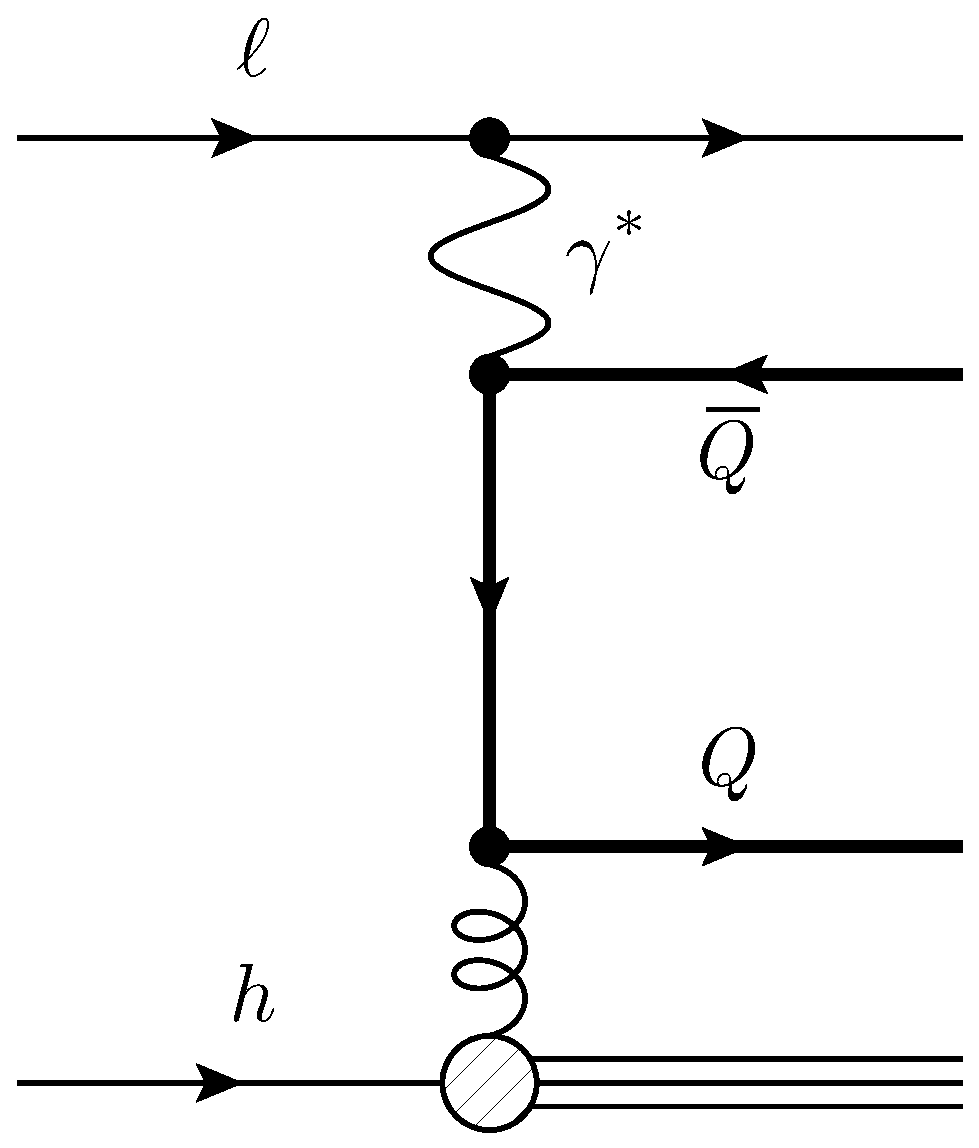
\includegraphics[width=.25\textwidth]{img/DIS.eps} &
\begin{itemize}
\item $S_h = (p+l_1)^2 = x\,y\,Q^2,\,x,\,y,$\\
$Q^2 = -q^2 = - (l_1-l_2)^2 \ll M_Z^2$
\item unpolarized cross section:\\
$\frac{d^2\sigma}{dx dy} = \frac{2\pi \alpha^2}{x y Q^2}\left(Y_+F_2(x,Q^2) - y^2F_L(x,Q^2)\right)$\\
$2xF_1(x,Q^2) = F_2(x,Q^2) - F_L(x,Q^2)$
\item polarized cross section:\\
$\frac{d^2\Delta\sigma}{dx dy} = \frac{4\pi \alpha^2}{x y Q^2}Y_-\cdot 2xg_1(x,Q^2)$
\item with $Y_\pm = 1 \pm (1-y)^2$
\item $[k=T]\to 2xF_1$, $[k=L]\to F_L$ and $[k=P]\to 2xg_1$
\end{itemize}
\end{tabular}
\end{frame}

%%%
\iffalse
\begin{frame}{Introduction - Experimental Setups}
\begin{center}
\newcolumntype{C}{>{\centering\arraybackslash} m{3.6cm} } 
\begin{tabular}{C|C|C}
\Pelectron-\APelectron-annihilation (SIA) & deep inelastic scattering (DIS) & Drell-Yan process (DY)\\
%SIA & DIS & DY\\
\hline
\vspace{3pt}
$\Pelectron+\APelectron \to \PaQ + X[\PQ]$ &
\vspace{3pt}
$\Pl+h \to \Pl' + \PaQ + X[\PQ]$ &
\vspace{3pt}
$h + h' \to \PaQ + X[\PQ]$ \\
\hline
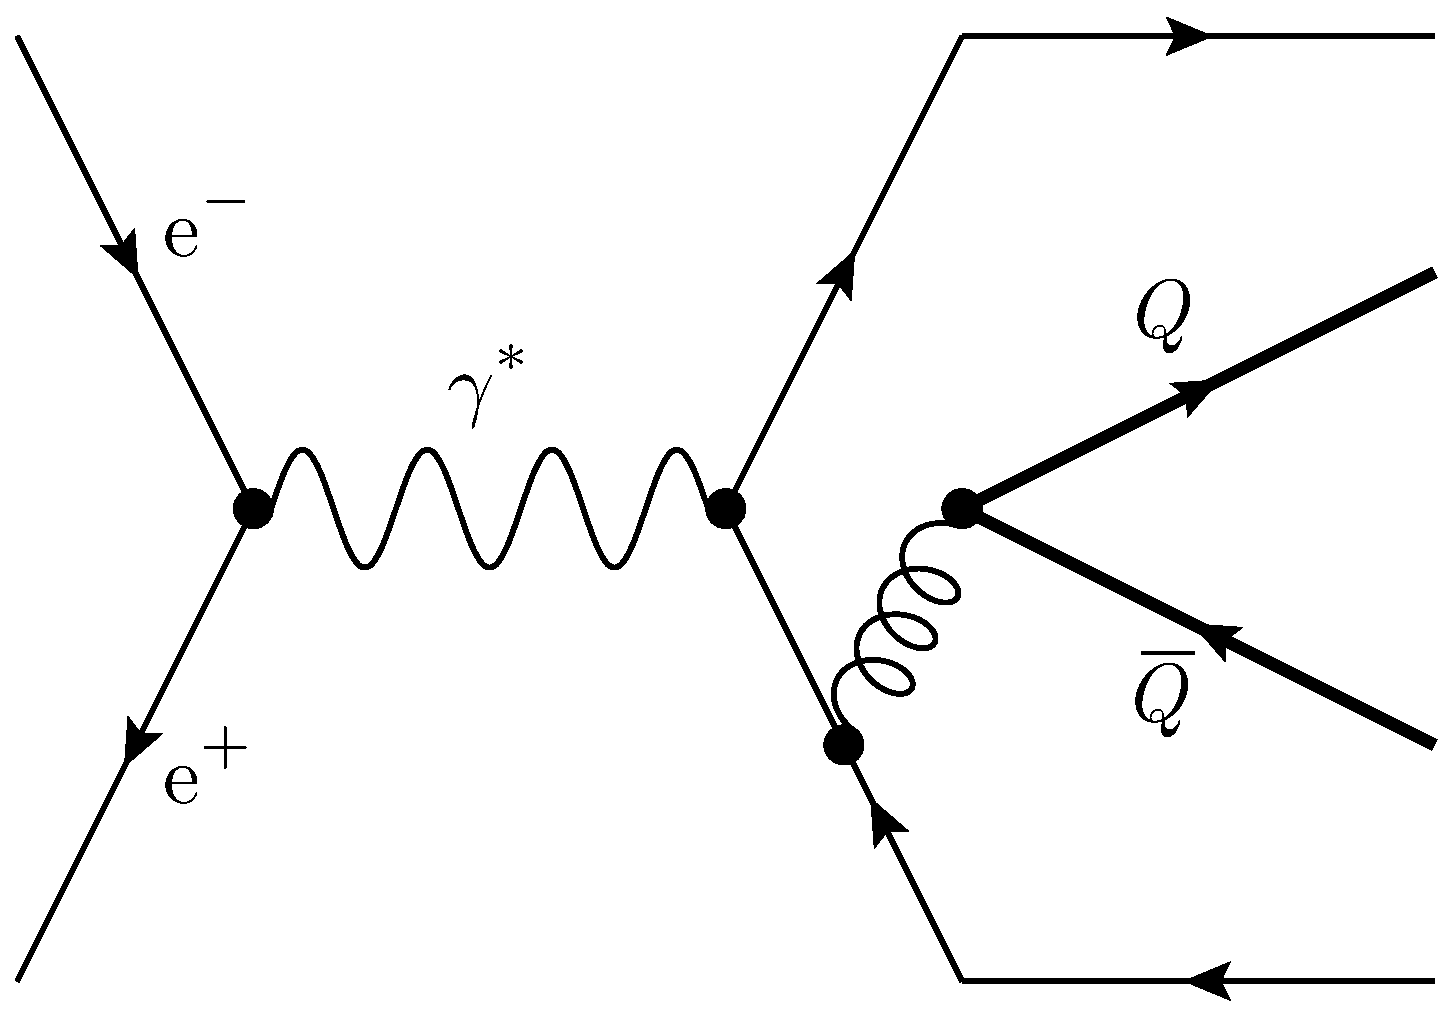
\includegraphics[width=.25\textwidth]{img/SIA.eps} & 
\vspace{.2cm}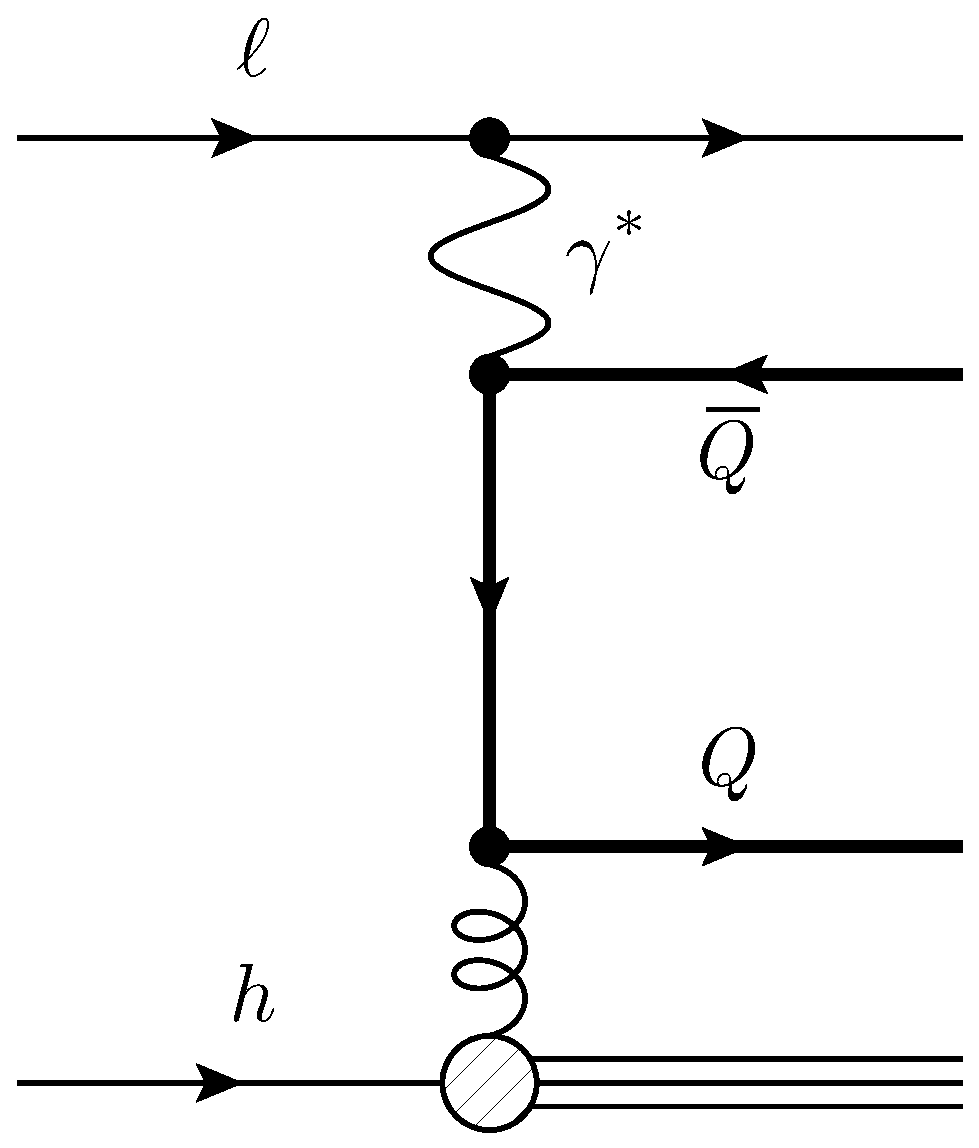
\includegraphics[width=.25\textwidth]{img/DIS.eps} & 
\vspace{.2cm}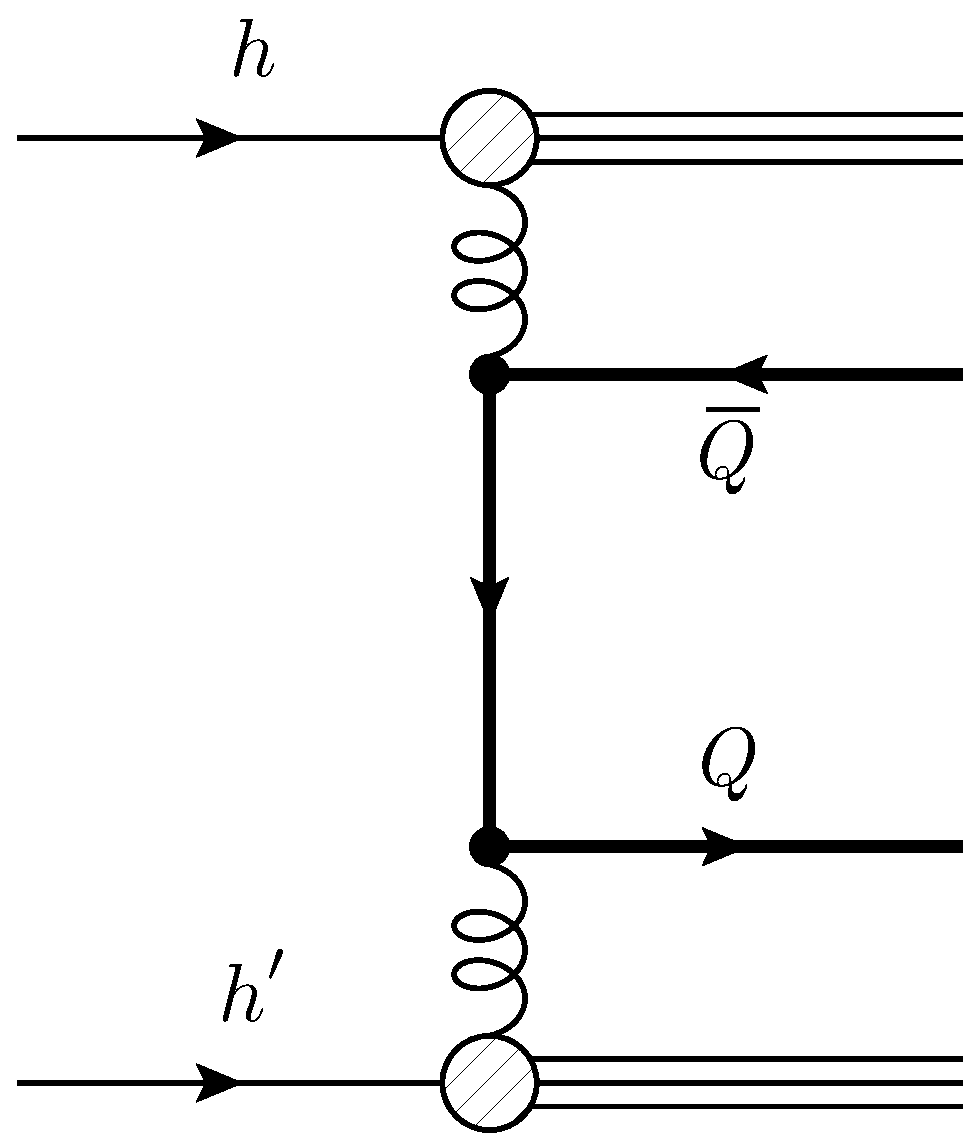
\includegraphics[width=.25\textwidth]{img/DY.eps} \\
\hline
LEP, ILC & \vspace{2pt} HERA, COMPASS, EIC & Tevatron, LHC\\
\hline
gluon & factorization & top, Higgs
\end{tabular}
\end{center}
\end{frame}

\begin{frame}{Introduction - Structure Functions}
\begin{align}
&\text{cross section (xs):}&\frac{d^2\sigma}{dx dy} &= \frac{2\pi y \alpha^2}{Q^4} L^{\mu\nu} W_{\mu\nu}\\
&\text{hadronic tensor:}&W_{\mu\nu} &= \left(-g_{\mu\nu} + \frac{q_\mu q_\nu}{q^2}\right) F_1(x,Q^2) + \frac{P_\mu P_\nu}{P\cdot q} F_2(x,Q^2) \nonumber\\
&& & \hspace{20pt} + i \epsilon_{\mu\nu\alpha\beta} \frac{q^{\alpha}S^{\beta}}{P\cdot q} g_1(x,Q^2)\\
&&F_L(x,Q^2) &= F_2(x,Q^2) - 2xF_1(x,Q^2)\\
&\text{unpolarized xs:}&\frac{d^2\sigma}{dx dy} &= \frac{2\pi \alpha^2}{x y Q^2}\left(Y_+F_2(x,Q^2) - y^2F_L(x,Q^2)\right)\\
&\text{polarized xs:}&\frac{d^2\Delta\sigma}{dx dy} &= \frac{4\pi \alpha^2}{x y Q^2}Y_-\cdot 2xg_1(x,Q^2)\\
&&Y_\pm &= 1 \pm (1-y)^2
\end{align}
\end{frame}
\fi
%%%
